\begin{figure*}
% graphic source https://docs.google.com/presentation/d/1CKU1Rtz8Vbk-Std3zFmzBcACf7EBj3amTTOAGKdBluQ
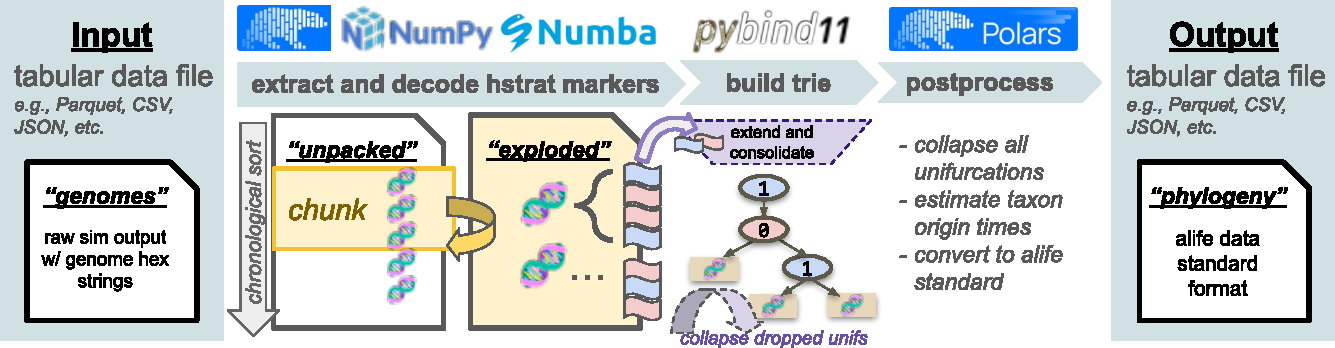
\includegraphics[width=\linewidth]{img/hstratpipeline.pdf}
\caption{%
\textbf{Phylogeny reconstruction pipeline.}
\small
Raw hexidecimal genome strings in ``genomes'' dataframe are segmented to ``unpack'' hstrat marker region.
Next, individual markers are decoded into ``exploded'' format.
Reconstruction progressively extends inferred trie one genome marker sequence at a time, with intermittent unifurcation cleanup to reduce memory usage.
Finally, trie is converted and saved as dataframe in alife data standard format.
Implementation leverages high-performance scientific computing libraries to achieve efficient operation on large datasets.
}
\label{fig:hstratpipeline}
\end{figure*}
